\documentclass{article}
\usepackage[utf8]{inputenc}
\usepackage{amssymb}
\usepackage{graphicx}
\usepackage{amsmath}

\title{CS350 HW6}
\author{Saeah Go}
\date{November 2021}

\begin{document}

\maketitle

\section{8.1.1}
What does dynamic programming have in common with divide-and-conquer? What is a principal difference between them? \\
\indent The similarity is that both break down a problem into multiple sub problems which are of similar type and then these problems are then combined for finding the final solution. \\
\indent In divide and conquer, the sub-problems are solved repeatedly many times. In dynamic programming, the sub-problems are computed once then stored in a table, so that next time the value is used from table instead of computing once more. \\
$\therefore$ time taken is faster than divide and conquer for computing the same problem. \\
\indent We have Fibonacci sequence as an example. With divide and conquer technique, we have $O(n^2)$ time complexity, and we have $O(n)$ for dynamic programming. 


\section{8.1.2}
Solve the instance 5, 1, 2, 10, 6 of the coin-row problem. \\
\indent We are given a row of n coins: 5, 1, 2, 10, 6. \\
The goal of the problem is to select coins with maximum profit with constraint no two adjacent coins are picked from these initial row. \\
$F(n)$ be maximum amount that could be picked up from the row of $n$ coins. \\
We have the following recurrence. \\
F(n) = max $\{C_n + F(n-2), F(n-1)\} \indent n > 1$ \\
F(0) = 0 F(1) = $C_1$ \\
{With the last coin - the max profit is} \\
{Without the last coin - the max profit is} \\
The above mentioned recurrence is obtained \\ \\
F[0] = 0, F[1] = $C_1$ = 5 \\
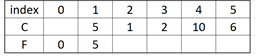
\includegraphics[scale = 0.7]{Picture1.png} \\
F[2] = max \{1 + 0, 5\} = 5 \\
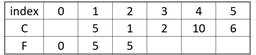
\includegraphics[scale = 0.7]{Picture2.png} \\
F[3] = max \{2 + 5, 5\} = 7 \\
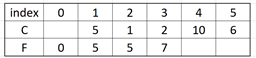
\includegraphics[scale = 0.7]{Picture3.png} \\
F[4] = max \{10 + 5, 7\} = 15 \\
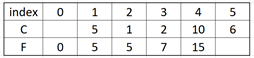
\includegraphics[scale = 0.7]{Picture4.png} \\
F[5] = max \{6 + 7, 15\} = 15 \\
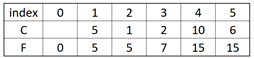
\includegraphics[scale = 0.7]{Picture5.png} \\
The maximum value of coins obtained will be 15.

\section{8.1.6}
\textit{Rod-cutting problem} Design a dynamic programming algorithm for the following problem. Find the maximum total sale price that can be obtained by cutting a rod of n units long into integer-length pieces if the sale price of a piece $i$ units long is $p_i$ for $i = 1, 2, . . . , n$. What are the time and space efficiencies of your algorithm? \\
Pseudocode: \\
int cutRod(int [] price, int n) \\
\{ \\
\indent val[] = array of size(n+1)\\
\indent val[0] = 0 \\
\indent for($i = 1$; $i <= n$; $i++$) \\
\indent \{ \\
\indent \indent max\_val = 0 \\ 
\indent \indent for($j=0$; $j < i$; $j++$) \\
\indent \indent \{ \\
\indent \indent \indent max\_val = maximum of (max\_val, price[j] + val[i-j-1]) \\
\indent \indent \} \\
\indent \indent val[i] = max\_val \\
\indent \} \\
\indent return val[n] \\
\} \\
Time efficiency of my algorithm: Since there are two nested for loops, the time complexity is $O(n^2)$. \\
Space efficiency of my algorithm: The space required to solve the problem is equal to the size of new array, so space time complexity is $O(n)$.


\section{8.2.2 a}
Write pseudocode of the bottom-up dynamic programming algorithm for the knapsack problem. \\
\indent A knapsack problem is a good technique in the dynamic programming. The knapsack is a collection $n$ items, each item with a weight and a value. Where $n$ is a number-of-items, Weights $w_1, \cdots , w_n$, Values $v_1, \cdots , v_n$ \\
\textbf{ALGORITHM} \textit{BottomUpKnapsack}(size, weights[$1, \cdots ,n$], values[$1, \cdots ,n$]) \\
\indent // Implements the bottom-up dynamic programming for knapsack problem 
\indent // Input: The first parameter "size" is a nonnegative integer indicating the number of items and the second parameter are an array of weights [$1, \cdots, n$] of $n$ items, and third parameter is an array of values [$1, \cdots, n$] of $n$ items. \\
\indent // Output: Table \textit{Matrix} [$0 \cdots Number of items, 0 \cdots size$] that contains the value of an optimal subset in \textit{Matrix}[$n, size$] from which the items of an optimal subset can be found. \\
\indent for $i \leftarrow 0$ to $n$ do \\
\indent \indent \textit{Matrix}[i, 0] $\leftarrow 0$ \\
\indent for $j \leftarrow 0$ to $size$ do \\
\indent \indent \textit{Matrix}[0, j] $\leftarrow 0$ \\
\indent for $i \leftarrow 1$ to $n$ do \\
\indent \indent for $j \leftarrow 0$ to $size$ do \\
\indent \indent \indent if $weights[i-1] \le j$ \\
\indent \indent \indent \indent \textit{Matrix}[i, j] $\leftarrow$ max(\textit{Matrix}[i-1, j], values[i-1] + \\
\indent \indent \indent \indent \indent \indent \indent \indent \indent \textit{Matrix}[i-1, j-weights[i-1]]) \\
\indent \indent \indent else \\
\indent \indent \indent \indent \textit{Matrix}[i, j] $\leftarrow$ \textit{Matrix}[i-1, j] \\
return \textit{Matrix}[n, size]

\section{8.2.3}
For the bottom-up dynamic programming algorithm for the knapsack problem, prove that \\
a. its time efficiency is $\Theta(nW)$. \\
b. its space efficiency is $\Theta(nW)$. \\
c. the time needed to find the composition of an optimal subset from a filled
dynamic programming table is $O(n)$.

a. Let there are $i$ items such that $1 \le i \le n$ and there weights are $w_1, \cdots, w_i$, and let the values of each item be $v_1, \cdots, v_i$, respectively. Suppose the capacity of the knapsack is $j$ such that $1 \le j \le W$. Suppose the optimal solution for the given items is $V[i,j]$. $V[i,j]$ is the item that gives most value per unit weight that means this the first item to be chosen at that moment for the $i$ items and knapsack with left weight $j$. \\
Using dynamic programming, divide the subsets into 2 different categories. In one category, put the optimal subset that contains $i^{th}$ item, and in second category put the optimal subset that does not contain $i^{th}$ item. \\
1. The optimal subset that does not contain $i^{th}$ item has value $V[i-1, j]$ \\
2. The subset that includes $i^{th}$ item, then the optimal subset will have $i^{th}$ item plus the optimal subset of $i-1$ items. Thus, the optimal subset is $v_i + V[i-1, j-w_i]$ \\
The optimal subset will be the maximum of two specified above. 
The recurrence relation for this problem is: \\
\begin{equation}
  V[i,j] =
    \begin{cases}
      max\{V[i-1, j], v_i + V[i-1, j-w_i]\} & \text{if $j-w_i \ge 0$} \\
      V[i-1, j] & \text{if $j-w_i < 0$}\\
    \end{cases}       
\end{equation}

The algorithm of the Knapsack problem fills a table with $n+1$ rows and $W+1$ columns, and takes $\Theta(1)$ to fill each cell by using the equation above. So it's time efficiency is: \\
$((n+1) * (W+1)) = nW + W + n + 1 \\
\indent \indent \indent \indent \indent \; \;  \; = \Theta(nW)$ \\ \\
\indent b. The algorithm of the Knapsack problem fills a table with $n+1$ rows and $W+1$ columns, and takes $\Theta(1)$ to fill each cell by using the equation above in the problem (a). \\
Thus the space efficiency is: \\
$((n+1) * (W+1)) = nW + W + n + 1 \\
\indent \indent \indent \indent \indent \; \;  \; = \Theta(nW)$ \\ \\
\indent c. In order to find the composition of an optimal subset, the algorithm compares values at no more than two cells in previous row. So its time efficiency class is: $O((n+1) + (W+1)) = O(n+W) = O(n)$


\end{document}
